\section{Videojuegos de construcción de ciudades}

Es un género dentro de los videojuegos de simulación, en el que los jugadores actúan como planificadores y líderes generales de una ciudad o pueblo, mirándola desde arriba, y siendo responsables de su crecimiento y estrategia de gestión. Los jugadores eligen la ubicación de los edificios y las características de gestión de la ciudad, como los salarios y las prioridades de trabajo, haciendo que la ciudad se desarrolle en consecuencia. \\

El exponente de este género es la serie de juegos de \textit{SimCity\texttrademark}, creados por el desarrollador de videojuegos Will Wright y padre de la saga \textit{The Sims\texttrademark}. Fue lanzado en 1989 y desde entonces, ha plateado las bases y ha servido de inspiración al resto de videojuegos dentro de este ámbito. A pesar de su fama, algunas malas decisiones en su última gran entrega (SimCity\texttrademark 2013) han hecho que haya perdido parte de su popularidad en favor de otros títulos.

Otro título dentro de este género es \textit{Cities: Skylines\textcopyright}, desarrollado por la productora filandesa \textit{Colossal Order}, y publicado por la editorial de videojuegos indie \textit{Paradox Interactive AB}. Pertenece a la serie de \textit{Cities in Motion\textcopyright}. Una de sus principales bazas con respecto a otros de su género es la simulación realista de tráfico, poniendo el foco en un sistema para entender los problemas en el diseño de la ciudad, y el uso de sistemas de transporte público para remediar problemas de congestión, que se ven potenciados en distintas expansiones del juego. Otra gran baza es que es altamente personalizable, pudiendo agregar desde mapas hasta modelos de objetos realistas, como edificios que existen en la realidad, coches de marcas conocidas, etc. Esto hace que esté entre el top 10 de títulos con más contenido creado por la comunidad del Workshop de Steam. En este proyecto vamos a utilizar esta característica de este título para poder crear un añadido que nos permita ejecutar nuestro programa lógico dentro del videojuego, y publicarlo posteriormente en Steam.

\section{Tecnologías}

Debido a las exigencias a la hora de desarrollar el proyecto, se ha optado por elegir un lenguaje de programación lógico sobre el que realizar la base declarativa del proyecto, ya que nos permitirá expresar las reglas de generación del mapa de forma matemática. También se ha escogido un segundo lenguaje multipropósito que nos permitirá desarrollar el plug-in que conectará nuestro programa lógico con el videojuego en cuestión.

\subsection{Answer Set Programming}\label{subsec:asp}

\textit{Answer Set Programming} (ASP) \cite{asp} es un paradigma enfocado a la resolución declarativa de problemas difíciles, combinando un lenguaje simple con el que modelar los problemas lógicos y herramientas de alto rendimiento para la resolución de estos. \textit{Answer Set Programming} está basado en modelos estables \cite{stablemodels}, que usa para definir la semántica declarativa mediante programas lógicos normales. A esto se añade a que incorpora lógica no monótona \cite{nonmonotonic}, que añade razonamiento por defecto. Con esto, \textit{Answer Set Programming} permite resolver problemas \textit{NP-hard} de forma uniforme. \\

Una regla de programación lógica tiene el siguiente aspecto:

\begin{equation}
	\underbrace{p}_{\text{\normalsize Cabeza}} \leftarrow \underbrace{q_1, \dotsc, q_m , \textit{not } q_{m+1} ,\dotsc, \textit{not } q_n}_{\text{\normalsize Cola}}.
\end{equation}

\hspace{1em}

o, en formato texto:

\begin{lstlisting}[label=lst:qreached]
p :- q1, ... , qm, not qm1, ..., not qn.
\end{lstlisting}

en donde $p$ y todos los $q_i$ son átomos, que son los elementos que pueden ser ciertos o falsos y los literales pueden ser tanto un átomo $s$ y su negación ($\text{not } s$). Intuitivamente, una regla es una justificación que establece o deriva que $p$ es verdad \textit{si} todos sus átomos a la derecha de la flecha $\leftarrow$ son ciertos. Por ejemplo, si suponemos la regla

\begin{equation}\label{eq:light}
	\textit{light\_on} \leftarrow \textit{power\_on}, \textit{not } broken.
\end{equation}

informalmente significa que se puede afirmar que la luz está encendida si se puede establecer que hay electricidad y no hay razón de pensar que la lámpara. Puede existir reglas que no tengan cuerpo,  como por ejemplo:

\begin{equation}\label{eq:power}
	\textit{power\_on} \leftarrow.
\end{equation}

Estas reglas se llaman hechos, ya que la cabeza es incondicionalmente cierta. Normalmente se omite la flecha $\leftarrow$. Los programas lógicos son una colección finita de reglas, en donde se expresa la ``justificación'' de un conjunto de átomos que pueden ser establecidos. Es importante señalar que \textit{not} no es el operador estándar de negación ($\lnot$), si no que significa que algo ``no es derivable''. Esto es lo que se llama negación por defecto \cite{negation}. Pensando en las dos reglas presentadas en \ref{eq:light} y \ref{eq:power}, \textit{power\_on} se puede derivar ya que es un hecho (\ref{eq:light}), mientras que \textit{broken} no porque no hay ninguna regla que lo derive. Esto nos permite derivar \textit{light\_on} (\ref{eq:power}), el cual sería el modelo estable. \\

Existe otro tipo de reglas, las cuales no tiene cabeza, es decir,

\begin{equation}
	\leftarrow B.
\end{equation}

Estas reglas se llaman \textit{constrains} o restricciones, y sirven para indicar que satisfacer \textit{B} es una contradicción. Así mismo es común que programas lógicos contengan el par de reglas

\begin{align}
	a &\leftarrow B, \textit{not } \bar{a}.\\
	\bar{a} &\leftarrow B, \textit{not } a.
\end{align}

en donde ni \textit{a} ni $\bar{a}$ aparecen en la cabeza de cualquier otra regla del programa, y B es una conjunción de literales. Esta regla aparece cuando se quiere referir tanto a un átomo \textit{a} como a su negación (estándar). Para representar este último, se introduce el nuevo átomo $\bar{a}$ y se incluye las dos reglas. Intuitivamente el rol de las reglas es seleccionar en caso de que \textit{B} se satisfaga. Estas reglas se pueden escribir como una regla \textit{choise} de la forma

\begin{align}
	\{a\} \leftarrow B.
\end{align}

En resumen, los problemas lógicos se reducen al cómputo de los modelos estables de un programa lógico dado, lo cual se hace mediante herramientas llamadas \textit{solvers}, que se encargan de utilizar diferentes técnicas para obtener un modelo estable final. \\

Para ello, se necesita que los programas lógicos estén expresados con variables libres. Como la forma de expresar un programa lógico en ASP es mediante un lenguaje de alto nivel con ciudadanos de primer orden, muchas de las variables están ligadas. Es por eso que, antes de resolver el programa, se usa unas herramientas llamadas \textit{grounders}, que permiten transformar el programa a su equivalente con variables libres. En la Figura \ref{fig:asp} se muestra el ciclo de ejecución de un programa ASP. \\

\begin{figure}[h]
	\centering
	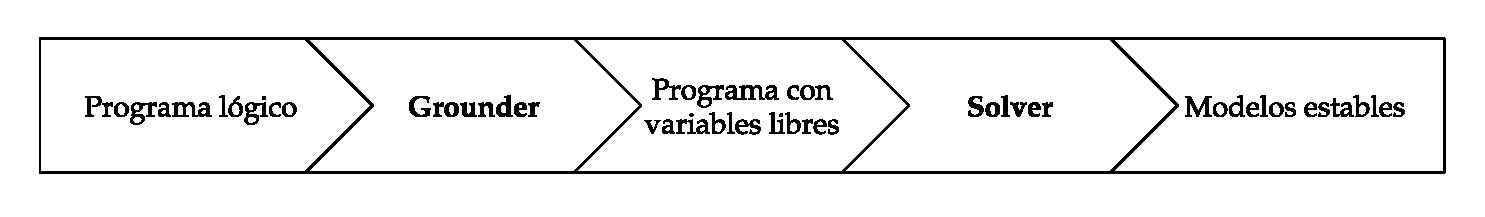
\includegraphics[height=4em]{images/ASP}
	\label{fig:asp}
	\caption{Ejemplo de ejecución de ASP}
\end{figure}

Unas de las herramientas más importantes de ASP son la de Potassco\footnote{http://potassco.org}, la cual son un conjunto de herramientas para ASP desarrolladas en la Universidad de Postdam. Contienen las herramientas fundamentales como un grounder llamado \textit{gringo}; un solver que es \textit{clasp}; y una herramienta que agluntina todo el sistema ASP, \textit{clingo}. Así mismo, añade más funcionalidades al lenguaje ASP, como puede ser al resolución iterativa, debido a que permite embeber otros lenguajes como Lua, el cual está explicado en la Sección \ref{subsec:lua}, o Python, que pueden interactuar con el programa escrito en ASP mediante la interfaz o \textit{API built-in} de clingo. \\

Estas herramientas serán claves a la hora de realizar este proyecto, ya que, como veremos más adelante, qué debido a la naturaleza de ASP, serán la base sobre la que se construirá todo el proyecto.

\subsection{.NET Framework}

TODO...

\section{Herramientas}

Aparte de las tecnologías usadas para la construcción del proyecto, se ha usado distintas herramientas que nos han servido a la hora de elaborar y desarrollar el sistema planteado.

\subsection{Visual Studio}

TODO

\subsection{Git}

Git\footnote{https://git-scm.com} es un sistema de control de versiones distribuido y de código abierto creado para la gestión de código fuente y desarrollo de software. Fue creado por Linus Trovalds como una alternativa libre y gratuita a BitKeeper para el desarrollo del kernel Linux por la comunidad. Está enfocado en la rapidez y eficiencia al procesar proyectos grandes, la integridad de datos, la seguridad mediante autentificación criptográfica y el fuerte soporte de un flujo de trabajo no lineal y distribuido. \\

Debido a estas características, Git es uno de los sistemas de control de versiones más importantes hoy en día, por lo que ha permitido que existan servicios de alojamiento en linea que incluyen esta herramienta:

\begin{itemize}
	\item GitLab\footnote{https://gitlab.com}, creado por dos programadores ucranianos y que hoy en día es gestionado por GitLab Inc. Es usado por organizaciones como Sony, IBM, NASA, CERN o GNOME Foundation. Permite realizar gratuitamente repositorios privados, gestionar grupos y realizar rastreo de \textit{issues} y funcionalidades de CI/CD.
	\item Phabricator\footnote{https://www.phacility.com}, creado por Facebook como herramienta interna que integra también Mercurial y Subversion. Actualmente es de código abierto y lo usan empresas como Blender, Cisco Systems, Dropbox o KDE.
	\item Bitbucket\footnote{https://bitbucket.org}, creado por Atlassian. Este sistema integra Mercurial desde sus inicios y Git desde 2011, y está pensado para ser integrado con el resto de productos como Atlassian como Jira, Confluence y Bamboo.
	\item GitHub\footnote{https://www.github.com}, creado por tres estudiantes estadounidenses, hoy en día es gestionado por GitHub Inc. empresa que fue adquirida por Microsoft en 2018. Permite realizar rastreo de \textit{bugs}, wikis, gestión de tareas y petición de funcionalidades. Es usado por empresas como Microsoft, Google, Travis CI, Bitnami, DigitalOcean y Unreal Engine. Con la popularidad de GitHub nacieron varios servicios, como el Education Program, que permite a estudiantes el acceso gratuito a herramientas de GitHub y de partners; Gist, que permite usar GitHub como un hosting de \textit{snippets} y GitHub Marketplace, que permite comprar servicios con los que aumentar las funcionalidades en los proyectos y que muchos de ellos son gestionados por partners.
\end{itemize}